\documentclass[12pt]{article}
\usepackage{ctex}
\usepackage{graphicx}
\usepackage{authblk}
\usepackage{subfigure}
\usepackage{caption}
\usepackage{amssymb}
\usepackage{graphicx, subfig}
\usepackage{float}
\usepackage{physics}
\usepackage{amsmath}
\usepackage{slashed}
\usepackage{geometry}
\captionsetup{font={small}}
\geometry{left=2.5cm,right=2.5cm,top=2.5cm,bottom=2.5cm}
\title{Chapter 6: Bose Systems}
\date{}
\author[1]{Tingyu Zhang}
\affil[1]{Department of Physics, Graduate School of Science, The University of Tokyo, 
Tokyo 113-0033, Japan}
\graphicspath{{figures/}}

\begin{document}

\maketitle
\section{\large Formulation}
The noninteracting ground state of $N$ bosons is given by
\begin{equation}\label{eq1}
    \ket*{\Phi_0(N)}=\ket*{N,0,0,\dots}
\end{equation}
where all the particles are in the lowest energy mode. If the creation and 
annihilation operators $a^\dagger_0$ and $a_0$ for the zero-momentum state are 
applied to the ground state, implies that 
\begin{equation}
    \begin{split}
        &a_0\ket*{\Phi_0(N)}=N^{\frac{1}{2}}\ket*{\Phi_0(N-1)}\\
        &a^\dagger_0\ket*{\Phi_0(N)}=(N+1)^{\frac{1}{2}}\ket*{\Phi_0(N+1)}.
    \end{split}
\end{equation}
Thus neither $a_0$ nor $a^\dagger_0$ annihilates the ground state. Unlike the 
case of fermions, the  operators $a^\dagger_0$ and $a_0$ for a Bose system 
multiply the ground state by $(N+1)^{\frac{1}{2}}$ or $N^{\frac{1}{2}}$, which 
is evidently large. We want to deal with intensive variables, therefore we 
define 
\begin{equation}
    \hat{\xi}_0=V^{-\frac{1}{2}}a_0\qquad
    \hat{\xi}^\dagger_0=V^{-\frac{1}{2}}a^\dagger_0
\end{equation}
with the following properties
\begin{equation}
    \begin{split}
        &\big[\hat{\xi}_0,\hat{\xi}^\dagger_0\big]=V^{-1}\\
        &\hat{\xi}_0\ket*{\Phi_0(N)}=\bigg(\frac{N}{V}\bigg)^{\frac{1}{2}}
        \ket*{\Phi_0(N-1)}\\
        &\hat{\xi}^\dagger_0\ket*{\Phi_0(N)}=\bigg(\frac{N+1}{V}\bigg)^{\frac{1}{2}}
        \ket*{\Phi_0(N+1)}.
    \end{split}
\end{equation}
The commutator of $\hat{\xi}_0$ and $\hat{\xi}^\dagger_0$ vanishes in the 
thermodynamic limit ($N\rightarrow\infty$, $V\rightarrow\infty$, 
$N/V\rightarrow\rm const$). Hence $\hat{\xi}_0$ and $\hat{\xi}^\dagger_0$ can 
be treat as $c$ numbers (Bogoliubov replacement) as long as we consider only systems where a finite fraction 
of the particles occupies the $\mathbf{k}=0$ mode.

In an interacting system, the potential energy makes
\begin{equation}
    \bra*{\Phi_0}\hat{\xi}^\dagger_0\hat{\xi}_0\ket*{\Phi_0}=N_0/V\equiv n_0
\end{equation}
less than the total density $n=N/V$. The boson field operator can be written as 
\begin{equation}\label{eq2}
    \hat{\psi}(\mathbf{x})=\xi_0+\sum_{\mathbf{k}\neq 0}V^{-1/2}
    e^{i\mathbf{k}\cdot\mathbf{x}}a_{\mathbf{k}}=\xi_0+\hat{\varphi}(\mathbf{x})
    =n_0^{1/2}+\hat{\varphi}(\mathbf{x})
\end{equation}
where the operator $\hat{\varphi}(\mathbf{x})$ has no zero-momentum components, and 
$\xi_0$ is a constant $c$ number. We calculate the commutator of 
$\hat{\varphi}$ and $\hat{\varphi}^\dagger$:
\begin{equation}\label{commutator}
    \begin{split}
        \big[\hat{\varphi}(\mathbf{x}),\hat{\varphi}^\dagger(\mathbf{x}')\big]&=V^{-1}
        \sum_{\mathbf{k}\neq 0}\sum_{\mathbf{k}'\neq 0}e^{i\mathbf{k}\cdot\mathbf{x}}
        a_{\mathbf{k}}e^{-i\mathbf{k}'\cdot\mathbf{x}'}a^\dagger_{\mathbf{k}'}
        -V^{-1}\sum_{\mathbf{k}\neq 0}\sum_{\mathbf{k}'\neq 0}e^{-i\mathbf{k}'\cdot\mathbf{x}'}
        a^\dagger_{\mathbf{k}'}e^{i\mathbf{k}\cdot\mathbf{x}}a_{\mathbf{k}}\\
        &=V^{-1}\sum_{\mathbf{k}\neq 0}\sum_{\mathbf{k}'\neq 0}e^{i(\mathbf{k}\cdot\mathbf{x}
        -\mathbf{k}'\cdot\mathbf{x}')}\big(a_{\mathbf{k}}a^\dagger_{\mathbf{k}'}-
        a^\dagger_{\mathbf{k}'}a_{\mathbf{k}}\big)\\
        &=V^{-1}\sum_{\mathbf{k}\neq 0}e^{i\mathbf{k}\cdot(\mathbf{x}-\mathbf{x}')}\\
        &=\delta^3(\mathbf{x}-\mathbf{x}')
    \end{split}
\end{equation}
which shows that the fields $\hat{\varphi}$ and $\hat{\varphi}^\dagger$ obey the 
canonical commutation relations.
Consider the potential energy
\begin{equation}\label{eq3}
    \hat{W}=\frac{1}{2}\int d^{3}xd^{3}x^{\prime}\hat{\psi}^\dagger(\mathbf{x})
    \hat{\psi}^\dagger\left(\mathbf{x}^{\prime}\right)W\left(\mathbf{x}-
    \mathbf{x}^{\prime}\right)\hat{\psi}\left(\mathbf{x}^{\prime}\right)\hat{\psi}
    (\mathbf{x})
\end{equation}
Substitute Eq.(\ref{eq2}) into Eq.(\ref{eq3}), we get eight parts 
\begin{align}
    &E_0=\frac{1}{2}n_0^2\int d^3xd^3x'W(\mathbf{x}-\mathbf{x}')\label{W0}\\
    &\hat{W}_{1}=\frac{1}{2}n_{0}\int d^{3}xd^{3}xW(\mathbf{x}-\mathbf{x}')
    \hat{\varphi}(\mathbf{x}')\hat{\varphi}(\mathbf{x})\label{W1}\\
    &\hat{W}_{2}=\frac{1}{2}n_{0}\int d^{3}xd^{3}x'\hat{\varphi}^\dagger(\mathbf{x}')
    \hat{\varphi}^\dagger(\mathbf{x})W(\mathbf{x}-\mathbf{x}')\\
    &\hat{W}_{3}=2\Big(\frac{1}{2}n_{0}\Big)\int d^{3}xd^{3}x'\hat{\varphi}^\dagger
    (\mathbf{x}')W(\mathbf{x}-\mathbf{x}')\hat{\varphi}(\mathbf{x})\\
    &\hat{W}_{4}=2\Big(\frac{1}{2}n_{0}\Big)\int d^{3}xd^{3}x'\hat{\varphi}^\dagger
    (\mathbf{x})W(\mathbf{x}-\mathbf{x}')\hat{\varphi}(\mathbf{x})\\
    &\hat{W}_{5}=2\Big(\frac{1}{2}n^{1/2}_{0}\Big)\int d^{3}xd^{3}x'\hat{\varphi}^\dagger
    (\mathbf{x})\hat{\varphi}^\dagger(\mathbf{x}')W(\mathbf{x}-\mathbf{x}')\hat{\varphi}(\mathbf{x})\\
    &\hat{W}_{6}=2\Big(\frac{1}{2}n^{1/2}_{0}\Big)\int d^{3}xd^{3}x'\hat{\varphi}^\dagger
    (\mathbf{x})W(\mathbf{x}-\mathbf{x}')\hat{\varphi}(\mathbf{x}')\hat{\varphi}(\mathbf{x})\\
    &\hat{W}_{7}=\frac{1}{2}\int d^{3}xd^{3}x'\hat{\varphi}^\dagger(\mathbf{x})
    \hat{\varphi}^\dagger(\mathbf{x}')W(\mathbf{x}-\mathbf{x}')\hat{\varphi}
    (\mathbf{x}')\hat{\varphi}(\mathbf{x})\label{W7}.
\end{align}
Note that
\begin{equation}
    \int d^{3}x\hat{\varphi}(\mathbf{x})=V^{-1/2}\sum_{\mathbf{k}\neq 0}a_{\mathbf{k}}
    \int d^{3}xe^{i\mathbf{k}\cdot\mathbf{x}}=V^{1/2}\sum_{\mathbf{k}\neq 0}
    a_{\mathbf{k}} \delta_{\mathbf{k} 0}=0.
\end{equation}
Therefore $\hat{W}$ contains no terms with only one particle out of the condensate.
$E_0$ is a $c$ number 
\begin{equation}
    E_0=\frac{1}{2}V^{-1}N_0^2W(0)
\end{equation}
that shifts the zero of energy but has no operator character.

Fig.\ref{img1} indicates the different processes in $\hat{W}$, where dash lines denotes 
particles in condensate $\xi_0$ or $\xi^\dagger_0$, wavy lines denotes the potential 
$W$ and solid lines denotes particles not in the condensate ($\hat{\varphi}$ or 
$\hat{\varphi}^\dagger$).
\begin{figure}[H]
    \centering
    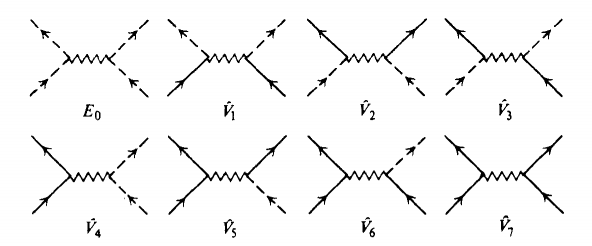
\includegraphics[width=13cm]{p1.png}
    \renewcommand{\figurename}{Fig.}
    \caption{Processes contained in $\hat{W}$ for bosons}
    \label{img1}
\end{figure}

In a noninteracting assembly, The ground state is given by Eq.(\ref{eq1}). We have no 
$a_0$ and $a^\dagger_0$ , therfore the \emph{vacuum} is 
\begin{equation}
    \ket*{0}\equiv\ket*{\Phi_0}=\ket*{N,0,0,\dots}.
\end{equation}
The vacuum expectation value of the total Hamiltonian:
\begin{equation}
    \bra*{0}\hat{H}\ket*{0}=E_0=\frac{1}{2}V^{-1}N_0^2W(0)
\end{equation}
which is the first-order contribution of the interaction to the ground-state energy.
The number operator 
\begin{equation}
    \begin{split}
        \hat{N}&=N_0+\int d^3x\hat{\varphi}^\dagger(\mathbf{x})\hat{\varphi}(\mathbf{x})
        =\sum_{\mathbf{k}\neq 0}\sum_{\mathbf{k}'\neq 0}V^{-1}\int d^3x
        e^{-i(\mathbf{k}-\mathbf{k}').\mathbf{x}}a_\mathbf{k}^\dagger a_{\mathbf{k}'}\\
        &=N_0+\sum_{\mathbf{k}\neq 0}a^\dagger_\mathbf{k}a_\mathbf{k}
    \end{split}
\end{equation}
$\hat{N}$ no longer commutes with the total Hamiltonian
\begin{equation}
    [\hat{T}+E_0+\hat{W}_1+\cdots+\hat{W}_7,\hat{N}]\neq 0
\end{equation}
As a result, the total number of particles is not a constant of the motion (caused by 
the condensate) but is 
determined as 
\begin{equation}
    N=N_0+\sum_{\mathbf{k}\neq 0}\langle a^\dagger_\mathbf{k}a_\mathbf{k}\rangle
\end{equation}
where the brackets denote the ground-state expectation value in the interacting system.
\section{The Thermodynamic Potential}
Return to the original Hamiltonian $\hat{H}=\hat{T}+\hat{W}$, in which $a_0$ and 
$a^\dagger_0$ are still operators. Let 
\begin{equation}
    \hat{K}=\hat{H}-\mu\hat{N}
\end{equation}
which commutes with $\hat{N}$ and has a set of eigenvectors and eigenvalues 
\begin{equation}
    \hat{K}\ket*{\Psi_j}=K_j\ket*{\Psi_j}
\end{equation}
The solution to an exact problem with an $N$ particles system is in a subspace of 
these eigenvectors. In this subspace, the ground state corresponds to the lowest 
eigenvalue of $\hat{K}$
\begin{equation}
    \hat{K}\ket*{\Psi_0(N)}=K(\mu,V,N)\ket*{\Psi_{0}(N)}=(E(V,N)-\mu N)\ket*{\Psi_0(N)}
\end{equation}
If we find a subspace in which $\mu$, $N$ and $V$ satisfy the thermodynamic relation 
\begin{equation}
    \mu=\frac{\partial E(V,N)}{\partial N},
\end{equation}
then 
\begin{equation}
    \frac{\partial K(\mu,V,N)}{\partial N}=\frac{\partial E(V,N)}{\partial N}-\mu=0.
\end{equation}
Therefore we can say the $K$ reaches its minimum at zero temperature and fixed 
$\mu$ and $V$.
\begin{equation}
    \bra*{\Psi_{0}(\mu)}\hat{K}\ket*{\Psi_{0}(\mu)}=\Omega(T=0,V,\mu)=
    \left.(E-\mu N)\right|_{T=0}
\end{equation} 
$\Omega$ is called the thermodynamic potential. $\ket*{\Psi_0(\mu)}$ therefore represents 
the equilibrium state of the assembly at fixed $T=0$, $\mu$ and $V$.
\subsection*{The Bogoliubov Prescription}
Replace $\hat{\xi}_0$ and $\hat{\xi}_0^\dagger$ with $c$ numbers 
\begin{equation}
    \hat{\xi}_0\rightarrow n_0^{1/2}\qquad\hat{\xi}_0^\dagger\rightarrow n_0^{1/2}
\end{equation}
\begin{equation}
    \Rightarrow \hat{N}\rightarrow N_0+\sum_{\mathbf{k}\neq0}a^\dagger_{\mathbf{k}}
    a_{\mathbf{k}}\equiv N_0+\hat{N}'
\end{equation}
and 
\begin{equation}
    \begin{split}
        \hat{K}&\rightarrow E_0-\mu N_0+\sum_{\mathbf{k}\neq0}(\epsilon_{\mathbf{k}}^0-\mu)
        a^\dagger_{\mathbf{k}}a_{\mathbf{k}}+\sum_{i=1}^7\hat{W}_i\\
        &\equiv E_0-\mu N_0+\hat{K}'.
    \end{split}
\end{equation}
In this way, we define $\hat{N}'$ and $\hat{K}'$. As all remaining annihilation operators 
annihilate the noninteracting ground state $\ket*{\Phi_0}$, it is also defined as the 
vacuum 
\begin{equation}
    \ket*{\Phi_0}\rightarrow \ket*{0}.
\end{equation}
The condition of thermodynamic equilibrium is 
\begin{equation}\label{equithermopotential}
    \left[\frac{\partial\Omega(T=0,V,\mu)}{\partial N_0}\right]_{V\mu}=0
\end{equation}
which is an implicit relation for $N_0(V,\mu)$.
\section{Green's Functions}
The Bogoliubov prescription gives the operator 
\begin{equation}
    \hat{K}=E_0-\mu N_0+\hat{K}'
\end{equation} 
where 
\begin{equation}\label{Kprime}
    \hat{K}'=\int d^3x\ \hat{\varphi}^\dagger(\mathbf{x})[T-\mu]\hat{\varphi}(\mathbf{x})
    +\sum_{i=1}^7\hat{W}_j
\end{equation}
$\hat{K}$ is hermitian and has a complete set of eigenfunctions. We define $\ket*{O}$ 
as the ground state of $\hat{K}$. The Heisenberg picture is defined as 
\begin{equation}\label{Heisenberg}
    \hat{O}_{K}(t)=e^{i\hat{K}t/\hbar}\hat{O}_{S}e^{-i\hat{K}t/\hbar}
    =e^{i\hat{K}'t/\hbar}\hat{O}_{S}e^{-i\hat{K}'t/\hbar}
\end{equation}
The field operator $\hat{\psi}(\mathbf{x})$ becomes 
\begin{equation}
    \begin{aligned}
        \hat{\psi}_K(\mathbf{x},t)&=e^{i\hat{K}'t/\hbar}\xi_{0} e^{-i\hat{K}'t/\hbar}
        +e^{i\hat{K}'t/\hbar}\hat{\varphi}(\mathbf{x})e^{-i\hat{K}'t/\hbar}\\
        &=\xi_0+\hat{\varphi}_{K}(x)=n_0^{1/2}+\hat{\varphi}_{K}(x)
        \end{aligned}
\end{equation}
showing the condensate part of $\hat{\psi}_K$ is independent on space and time.
The single particle Green's function is defined as 
\begin{equation}
    \begin{split}
        iG(x,y)&=\frac{\bra*{O}T\big[\big(\xi_0+\hat{\varphi}_K(x)\big)\big(\xi_0+
        \hat{\varphi}^\dagger_K(x)\big)\big]\ket*{O}}{\bra*{O}\ket*{O}}\\
        &=n_0+n_0^{1/2}\frac{\bra*{O}\hat{\varphi}_K(x)+\hat{\varphi}^\dagger_K(x)
        \ket*{O}}{\bra*{O}\ket*{O}}+\frac{\bra*{O}T\big[\hat{\varphi}_K(x)\hat{\varphi}
        ^\dagger_K(x)\big]\ket*{O}}{\bra*{O}\ket*{O}}.
    \end{split}\label{Green}
\end{equation}
different from fermion assembly, the signature factor for all time orderings is $+1$. 
Obviously, the second term in the r.h.s of Eq.(\ref{Green}) vanishes. As a result, 
$G(x,y)$ takes the form 
\begin{align}
    &iG(x,y)=n_0+iG'(x,y)\\
    &iG'(x,y)=\frac{\bra*{O}T\big[\hat{\varphi}_K(x)\hat{\varphi}^\dagger_K(x)\big]
    \ket*{O}}{\bra*{O}\ket*{O}}.
\end{align}
$G'(x,y)$ refers to the noncondensate. The expectation value of $\hat{N}$ can be 
written as 
\begin{equation}\label{N}
    N=\langle\hat{N}\rangle=N_0+V\int \frac{d^4q}{(2\pi)^4}\ iG'(q)e^{iq_0\eta}
\end{equation}
where $q=(q_0,\mathbf{q})$ and the limit $\eta\rightarrow 0^{+}$ is implicit. The 
kinetic energy can be written as 
\begin{equation}
    T=\langle\hat{T}\rangle=V\int \frac{d^4q}{(2\pi)^4}\frac{\hbar^2\mathbf{q}^2}
    {2m}iG'(q)e^{iq_0\eta}
\end{equation}
Acoording to Eq.(\ref{Heisenberg}), we can write
\begin{equation}\label{HeisenbergEq}
    i\hbar\frac{\partial\hat{\varphi}_K(x)}{\partial t}=[\hat{\varphi}_K(x),\hat{K}'].
\end{equation}
Below are some simple calculations:

\noindent\hrulefill
\begin{equation}
    \begin{split}
        \big[\hat{\varphi}_K(\mathbf{x}),\hat{K}'\big]&=e^{i\hat{K}'t/\hbar}
        \hat{\varphi}(\mathbf{x})e^{-i\hat{K}'t/\hbar}\hat{K}'-\hat{K}'e^{i\hat{K}'t
        /\hbar}\hat{\varphi}(\mathbf{x})e^{-i\hat{K}'t/\hbar}\\
        &=e^{i\hat{K}'t/\hbar}\big[\hat{\varphi}(\mathbf{x}),\hat{K}'\big]
        e^{-i\hat{K}'t/\hbar}.
    \end{split}
\end{equation}
Then, according to Eq.(\ref{commutator}) and Eq.(\ref{Kprime}),
\begin{equation}\label{cmK}
    \begin{split}
        \big[\hat{\varphi}(\mathbf{x}),\hat{K}'\big]&=\int d^3x'\big[\hat{\varphi}
        (\mathbf{x}),\hat{\varphi}^\dagger(\mathbf{x}')\big](T-\mu)\hat{\varphi}
        (\mathbf{x}')+\Big[\hat{\varphi}(\mathbf{x}),\sum_{i=1}^7\hat{W}_i\Big]\\
        &=(T-\mu)\hat{\varphi}(\mathbf{x})+\sum_{i=1}^7\big[\hat{\varphi}(\mathbf{x}),
        \hat{W}_i\big].
    \end{split}
\end{equation}
With Eq.(\ref{W1}) to Eq.(\ref{W7}), we can write 
\begin{equation}\label{cm1}
    \big[\hat{\varphi}(\mathbf{x}),\hat{W}_1\big]=0
\end{equation}
\begin{equation}
    \begin{split}
        \big[\hat{\varphi}(\mathbf{x}),\hat{W}_2\big]=&\frac{1}{2}n_0\int d^3x'
        \int d^3x''\big[\hat{\varphi}(\mathbf{x})\hat{\varphi}^\dagger(\mathbf{x}')
        \hat{\varphi}^\dagger(\mathbf{x}'')-\hat{\varphi}^\dagger(\mathbf{x}')
        \hat{\varphi}^\dagger(\mathbf{x}'')\hat{\varphi}(\mathbf{x})\big]W(\mathbf{x}'
        -\mathbf{x}'')\\
        =&\frac{1}{2}n_0\int d^3x'\int d^3x''\big\{\big[\hat{\varphi}(\mathbf{x}),
        \hat{\varphi}^\dagger(\mathbf{x}')\big]\hat{\varphi}^\dagger(\mathbf{x}'')
        +\hat{\varphi}^\dagger(\mathbf{x}')\big[\hat{\varphi}(\mathbf{x}),
        \hat{\varphi}^\dagger(\mathbf{x}'')\big]\big\}W(\mathbf{x}'-\mathbf{x}'')\\
        =&\frac{1}{2}n_0\int d^3x'\int d^3x''\big\{\delta^3(\mathbf{x}-\mathbf{x}')
        \hat{\varphi}^\dagger(\mathbf{x}'')+\hat{\varphi}^\dagger(\mathbf{x}')
        \delta^3(\mathbf{x}-\mathbf{x}'')\big\}W(\mathbf{x}'-\mathbf{x}'')\\
        =&2\Big(\frac{1}{2}n_0\Big)\int d^3x'\hat{\varphi}^\dagger(\mathbf{x}')
        W(\mathbf{x}-\mathbf{x}')
    \end{split}
\end{equation}
\begin{equation}
    \begin{split}
        \big[\hat{\varphi}(\mathbf{x}),\hat{W}_3\big]&=2\Big(\frac{1}{2}n_0\Big)
        \int d^3x'\int d^3x''\big[\hat{\varphi}(\mathbf{x}),\hat{\varphi}^\dagger
        (\mathbf{x}'')\big]W(\mathbf{x}'-\mathbf{x}'')\hat{\varphi}(\mathbf{x}')\\
        &=2\Big(\frac{1}{2}n_0\Big)\int d^3x'W(\mathbf{x}-\mathbf{x}')\hat{\varphi}
        (\mathbf{x}')
    \end{split}
\end{equation}
\begin{equation}
    \begin{split}
        \big[\hat{\varphi}(\mathbf{x}),\hat{W}_4\big]&=2\Big(\frac{1}{2}n_0\Big)
        \int d^3x'\int d^3x''\big[\hat{\varphi}(\mathbf{x}),\hat{\varphi}^\dagger
        (\mathbf{x}')\big]W(\mathbf{x}'-\mathbf{x}'')\hat{\varphi}(\mathbf{x}')\\
        &=2\Big(\frac{1}{2}n_0\Big)\int d^3x'W(\mathbf{x}-\mathbf{x}')\hat{\varphi}
        (\mathbf{x})
    \end{split}
\end{equation}
\begin{equation}
    \begin{split}
        \big[\hat{\varphi}(\mathbf{x}),\hat{W}_5\big]=&2\Big(\frac{1}{2}n_0^{1/2}\Big)
        \int d^3x'\int d^3x''\big\{\big[\hat{\varphi}(\mathbf{x}),\hat{\varphi}
        ^\dagger(\mathbf{x}')\big]\hat{\varphi}^\dagger(\mathbf{x}'')\\
        &+\hat{\varphi}^\dagger(\mathbf{x}')\big[\hat{\varphi}(\mathbf{x}),
        \hat{\varphi}^\dagger(\mathbf{x}'')\big]\big\}W(\mathbf{x}'-\mathbf{x}'')
        \hat{\varphi}(\mathbf{x}')\\
        =&2\Big(\frac{1}{2}n_0^{1/2}\Big)\int d^3x'\hat{\varphi}^\dagger(\mathbf{x}')
        W(\mathbf{x}-\mathbf{x}')\big[\hat{\varphi}(\mathbf{x})+\hat{\varphi}
        (\mathbf{x}')\big]
    \end{split}
\end{equation}
\begin{equation}
    \begin{split}
        \big[\hat{\varphi}(\mathbf{x}),\hat{W}_6\big]&=2\Big(\frac{1}{2}n_0^{1/2}\Big)
        \int d^3x'\int d^3x''\big[\hat{\varphi}(\mathbf{x}),\hat{\varphi}^\dagger
        (\mathbf{x}')\big]W(\mathbf{x}'-\mathbf{x}'')\hat{\varphi}(\mathbf{x}'')
        \hat{\varphi}(\mathbf{x}')\\
        &=2\Big(\frac{1}{2}n_0^{1/2}\Big)\int d^3x'W(\mathbf{x}-\mathbf{x}')
        \hat{\varphi}(\mathbf{x}')\hat{\varphi}(\mathbf{x})
    \end{split}
\end{equation}
\begin{equation}\label{cm7}
    \begin{split}
        \big[\hat{\varphi}(\mathbf{x}),\hat{W}_7\big]&=\frac{1}{2}\int d^3x'\int
        d^3x''\big\{\big[\hat{\varphi}(\mathbf{x}),\hat{\varphi}^\dagger(\mathbf{x}')
        \big]\hat{\varphi}^\dagger(\mathbf{x}'')\\
        &+\hat{\varphi}^\dagger(\mathbf{x}')\big[\hat{\varphi}(\mathbf{x}),
        \hat{\varphi}^\dagger(\mathbf{x}'')\big]\big\}W(\mathbf{x}'-\mathbf{x}'')
        \hat{\varphi}(\mathbf{x}'')\hat{\varphi}(\mathbf{x}')\\
        &=\int d^3x'\hat{\varphi}^\dagger(\mathbf{x}')W(\mathbf{x}-\mathbf{x}')
        \hat{\varphi}(\mathbf{x}')\hat{\varphi}(\mathbf{x}).
    \end{split}
\end{equation}
With Eq.(\ref{HeisenbergEq}) to Eq.(\ref{cm7}), we can then wirte the following 
equations
\begin{equation}
    \int d^3x\ \hat{\varphi}_K^\dagger(\mathbf{x})\Big(i\hbar\frac{\partial}{\partial 
    t}-T+\mu\Big)\hat{\varphi}_K(\mathbf{x})=2\hat{w}_2+\hat{W}_3+\hat{W}_4+2\hat{W}_5
    +\hat{W}_6+2\hat{W}_7
\end{equation}
and its adjoint 
\begin{equation}
    \int d^3x\Big[\Big(-i\hbar\frac{\partial}{\partial t}-T+\mu\Big)\hat{\varphi}_K
    ^\dagger(\mathbf{x})\Big]\hat{\varphi}_K(\mathbf{x})=2\hat{W}_1+\hat{W}_3+
    \hat{W}_4+\hat{W}_5+2\hat{U}_6+2\hat{W}_7.
\end{equation}
Their average is 
\begin{equation}\label{average}
    \begin{aligned}
        \frac{1}{2} \int d^{3} x\Big\{\hat{\varphi}_{K}^{\dagger}(x)&\Big(i\hbar
        \frac{\partial}{\partial t}-T+\mu\Big)\hat{\varphi}_{K}(x)+\Big[\Big(-i\hbar
        \frac{\partial}{\partial t}-T+\mu\Big)\hat{\varphi}_{k}^{\dagger}(x)\Big]
        \hat{\varphi}_{K}(x)\Big\} \\
        =&\big(\hat{W}_1+\hat{W}_2+\hat{W}_3+\hat{W}_4\big)+\frac{3}{2}\big(\hat{W}_5
        +\hat{W}_6\big)+2\hat{W}_7\\
        =&2\hat{W}-n_0\frac{\partial\hat{W}}{\partial n_0}
        \end{aligned}
\end{equation}
where $\hat{W}$ is the total interaction energy 
\begin{equation}
    \hat{W}=E_0+\sum_{i=1}^7\hat{W}_i
\end{equation}
\hrulefill

The ground state expectation value of Eq.(\ref{average}) is 
\begin{equation}\label{VGreen}
    \begin{split}
        \int d^3x\lim _{x'\rightarrow x,t'\rightarrow t^+}\frac{1}{2}&\Big[i
        \hbar\frac{\partial}{\partial t}-T(\mathbf{x})+\mu-i\hbar\frac{\partial}
        {\partial t'}-T(\mathbf{x}')+\mu\Big]iG'(\mathbf{x}t,\mathbf{x}'t')\\
        =&2\langle\hat{W}\rangle-n_0\bigg\langle\frac{\partial\hat{W}}{\partial n_0}
        \bigg\rangle,
        \end{split}
\end{equation}
thereby expressing $\langle\hat{W}\rangle$ in terms of $G'$. The thermodynamic 
potential at $T=0$ is 
\begin{equation}
    \Omega(T=0,V,\mu,N_0)=\bra*{O}\hat{K}\ket*{O}
\end{equation}
Where $\ket*{O}$ is assumed normalized. And the relation for thermodynamic equilibrium 
Eq.(\ref{equithermopotential}) remains unchanged.
\begin{equation}
    \Big(\frac{\partial\Omega}{\partial N_0}\Big)_{V\mu}=\frac{\partial}
    {\partial N_0}\bra*{O}\hat{K}\ket*{O}=\bra*{O}\frac{\partial \hat{K}}{\partial
    N_0}\ket*{O}=\bra*{O}\frac{\partial \hat{W}}{\partial N_0}-\mu\ket*{O}=0,
\end{equation}
giving the chemical potential 
\begin{equation}\label{equichemical}
    \mu=\bra*{O}\frac{\partial \hat{W}}{\partial N_0}\ket*{O}.
\end{equation}
Combinating of Eqs.(\ref{N}), (\ref{VGreen}), and (\ref{equichemical}) yields
\begin{equation}
    \begin{split}
        \langle\hat{W}\rangle=&\frac{1}{2}\int d^3x\lim _{x'\rightarrow x,t'
        \rightarrow t^+}\frac{1}{2}\Big[i\hbar\frac{\partial}{\partial t}-T
        (\mathbf{x})+\mu-i\hbar\frac{\partial}{\partial t'}-T(\mathbf{x}')+\mu\Big]
        iG'(\mathbf{x}t,\mathbf{x}'t')\\
        &+\frac{1}{2}n_0\Big\langle\frac{\partial\hat{W}}{\partial n_0}\Big\rangle\\
        =&\frac{1}{2}\int d^3x\lim _{x'\rightarrow x,t'\rightarrow t^+}\Big[\frac{1}
        {2}i\hbar\Big(\frac{\partial}{\partial t}-\frac{\partial}{\partial t'}\Big)-
        \frac{1}{2}\big(T(\mathbf{x})+T(\mathbf{x}')\big)+\mu\Big]iG'(\mathbf{x}t,
        \mathbf{x}'t')+\frac{1}{2}\mu N_0\\
        =&\frac{1}{2}\int d^3x\lim _{x'\rightarrow x,t'\rightarrow t^+}\Big[\frac{1}
        {2}i\hbar\Big(\frac{\partial}{\partial t}-\frac{\partial}{\partial t'}\Big)-
        T(\mathbf{x})\Big]iG'(x,x')+\frac{1}{2}\mu N
    \end{split}
\end{equation}
\begin{equation}
    E=\langle\hat{T}+\hat{W}\rangle=\frac{1}{2}\mu N+\frac{1}{2}\int d^3x\lim _{x'
    \rightarrow x,t'\rightarrow t^+}\Big[\frac{1}{2}i\hbar\Big(\frac{\partial}
    {\partial t}-\frac{\partial}{\partial t'}\Big)+T(\mathbf{x})\Big]iG'(x,x').
\end{equation}
The total energy can be rewritten with a Fourier transformation 
\begin{equation}\label{E}
    E=\frac{1}{2}\mu N+\frac{1}{2}V\int\frac{d^4q}{(2\pi)^4}\Big(\hbar q_0+
    \frac{\hbar^2\mathbf{q}^2}{2m}\Big)iG'(q)e^{iq_0\eta}
\end{equation}
The thermodynamic potential
\begin{equation}
    \Omega(T=0)=E-\mu N=\frac{1}{2}V\int\frac{d^4q}{(2\pi)^4}\Big(\hbar q_0+
    \frac{\hbar^2\mathbf{q}^2}{2m}\Big)iG'(q)e^{iq_0\eta}-\frac{1}{2}\mu N
\end{equation}
\subsection*{Anomalous Green's function}
As the Bogoliubov Prescription, we consider the whole condensed particles in a system 
as a large source of particles. It can create and absorb particles, which cause the 
nonconservation of the particle number. Therefore, apart from the single particle 
Green's function we introduced above, we also have two anomalous Green's function 
that don't obey the conservation of particle number:
\begin{subequations}
    \begin{align}
        &iG'_{12}(x,y)=\frac{\bra*{O}T\big[\hat{\varphi}_K(x)\hat{\varphi}_K(y)\big]
        \ket*{O}}{\braket*{O}{O}}\label{Za}\\
        &iG'_{12}(x,y)=\frac{\bra*{O}T\big[\hat{\varphi}^\dagger_K(x)\hat{\varphi}^\dagger_K(y)
        \big]\ket*{O}}{\braket*{O}{O}}\label{Zb},
    \end{align}
\end{subequations}
which representing the appearance and disappearance of two particles from the 
condensate. Obviusly, they are symmetric under the exchange of $x$ and $y$, 
\begin{equation}
    G_{12}'(x,y)=G_{12}'(y,x) \qquad G_{21}'(x,y)=G_{21}'(y,x),
\end{equation}
which means 
\begin{equation}
    G_{12}'(p)=G_{12}'(-p) \qquad G_{21}'(p)=G_{21}'(-p).
\end{equation}
Therefore, we introduce a $2\times 2$ matrix Green's function 
\begin{equation}
    i\mathbf{G}'(x,y)=\frac{\bra*{O}T\big[\hat{\Phi}_K(x)\hat{\Phi}_K^\dagger(y)\big]
        \ket*{O}}{\braket*{O}{O}},
\end{equation}
where 
\begin{equation}
    \hat{\Phi}_K(x)=\left(\begin{matrix}
        \hat{\varphi}_K(x)\\
        \hat{\varphi}^\dagger_K(x)
    \end{matrix}\right).\qquad
    \mathbf{G}'(p)=\left(\begin{matrix}
        G'(p) &G'_{12}(p)\\
        G'_{21}(p) &G'(-p)
    \end{matrix}\right)
\end{equation}

\section{Perturbation Theory}
\subsection*{Interaction picture}
We introduce $\hat{K}_0$, which is $\hat{K}'$ with the interaction term 
$\sum_{i}^7W_i$ eliminated.
\begin{equation}
    \hat{K}_0=E_0-\mu N_0+\hat{K}'_0
\end{equation}
where
\begin{equation}
    \hat{K}'_0=\hat{T}-\mu\hat{N}'=\int d^3x\ \hat{\varphi}^\dagger(\mathbf{x})[T-\mu]
    \hat{\varphi}(\mathbf{x}).
\end{equation}
The interaction picture is 
\begin{equation}
    \hat{O}_I(t)=e^{i\hat{K}_0t/\hbar}\hat{O}_se^{-i\hat{K}_0t/\hbar}=
    e^{i\hat{K}'_0t/\hbar}\hat{O}_se^{-i\hat{K}'_0t/\hbar}
\end{equation}
The unitary operator 
\begin{equation}
    \hat{U}(t,t_0)=e^{i\hat{K}'_0t/\hbar}e^{-i\hat{K}'(t-t_0)/\hbar}e^{-i\hat{K}'_0
    t/\hbar}
\end{equation}
which defines the evolution of states in the interaction picture. This operator obeys 
\begin{equation}
    \begin{aligned}
        i \hbar \frac{\partial \hat{U}(t,t_0)}{\partial t}&=e^{i\hat{K}'_0t/\hbar}
        \left(\hat{K}'-\hat{K}_0'\right)e^{-t \hat{K}'_0t/\hbar}\hat{U}(t,t_0)\\
        &=e^{t\hat{K}'_0t/\hbar}\hat{K}_1e^{-i\hat{K}'_0t/\hbar}\hat{U}(t,t_0) \\
        &=\hat{K}_1(t)\hat{U}(t,t_0)
        \end{aligned}
\end{equation}
where 
\begin{equation}
    \hat{K}_1=\sum_{i=1}^7\hat{W}_i\qquad\hat{K}=\hat{K}_0+\hat{K}_1.
\end{equation}
\begin{equation}
    [\hat{K}_0,\hat{N}]=0.
\end{equation}
Thus the ground state $\ket*{0}$ of $\hat{K}_0$ is a state of conserved number of 
particles. (Obviously, since $\hat{K}_0$ has no interaction parts that changes the 
number of particles in $\mathbf{k}\neq0$ modes.) After some manipulations, we 
can expand the single particle Green's function in series:
\begin{equation}
    \begin{aligned}
        i G^{\prime}(x, y)=\sum_{m=0}^{\infty}\left(\frac{-i}{\hbar}\right)^{m}
        \frac{1}{m !} \int_{-\infty}^{\infty} d t_{1}\cdots&\int_{-\infty}^{\infty} d t_{m} \\
        \times\bra*{0} T\left[\hat{K}_{1}\left(t_{1}\right)\cdots\right.&\left.
        \hat{K}_{1}\left(t_{m}\right)\hat{\varphi}_{I}(x) \hat{\varphi}_{I}^{\dagger}
        (y)\right]\ket*{0}_{\text {connected }}.
        \end{aligned}
\end{equation}
The free Green's function is
\begin{equation}
    iG^0(x,y)=\bra*{0}T\big[\hat{\varphi}_I(x)\hat{\varphi}^\dagger_I(y)\big]\ket*{0}.
\end{equation}
By performing Fourier transform on it, we have 
\begin{equation}
    G^0(\mathbf{q},t-t')=-i\Theta(t-t')e^{-i(\epsilon_{\mathbf{q}}-\mu)(t-t')}
\end{equation}
and 
\begin{equation}
    G^0(q)=\frac{1}{q_0-\omega_{\mathbf{q}}+\mu/\hbar+i\eta}
\end{equation}
where $\omega_{\mathbf{q}}=\epsilon_{\mathbf{q}}/\hbar$.
\subsection*{Some detailed calculations}
\noindent\hrulefill
\begin{equation}
    \begin{split}
        iG^0(x,y)&=\bra*{0}T\big[\hat{\varphi}_I(x)\hat{\varphi}^\dagger_I(y)\big]
        \ket*{0}\\
        &=\Theta(t-t')\bra*{0}e^{iK_0t/\hbar}\hat{\varphi}(\mathbf{x})e^{-iK_0t/\hbar}
        e^{iK_0t'/\hbar}\hat{\varphi}(\mathbf{y})e^{-iK_0t'/\hbar}\ket*{0}\\
        &=V^{-1}\Theta(t-t')\sum_{\mathbf{k}\neq 0}\sum_{\mathbf{k}'\neq 0}e^{i
        \mathbf{k}\cdot\mathbf{x}}a_{\mathbf{k}}e^{-iK_0t/\hbar}e^{iK_0t'/\hbar}
        e^{-i\mathbf{k}'\cdot\mathbf{y}}a_{\mathbf{k}'}\ket*{0}\\
        &=V^{-1}\Theta(t-t')\sum_{\mathbf{k}\neq 0}\sum_{\mathbf{k}'\neq 0}\bra*{
        \mathbf{k}}e^{-i(\epsilon_{\mathbf{k}}-\mu)t/\hbar}e^{i(\epsilon_{\mathbf{k}'}
        -\mu)t'/\hbar}\ket*{\mathbf{k}'}e^{i(\mathbf{k}\cdot\mathbf{x}-\mathbf{k}'
        \cdot\mathbf{y})}\\
        &=V^{-1}\Theta(t-t')\sum_{\mathbf{k}\neq 0}e^{-i(\epsilon_{\mathbf{k}}-\mu)
        (t-t')/\hbar}e^{i\mathbf{k}\cdot(\mathbf{x}-\mathbf{y})}.
    \end{split}
\end{equation}
Let $\mathbf{r}=\mathbf{x}-\mathbf{y}$ and perform the Fourier transform:
\begin{equation}
    \begin{split}
        G^0(\mathbf{q},t-t')&=V\int d^3r\ G^0(x,y)e^{-i\mathbf{q}\cdot\mathbf{r}}\\
        &=-i\Theta(t-t')\sum_{\mathbf{k}\neq 0}\int d^3r\ e^{-i(\epsilon_{\mathbf{k}}
        -\mu)(t-t')/\hbar}e^{i\mathbf{k}\cdot\mathbf{r}}e^{-i\mathbf{q}\cdot\mathbf{r}}\\
        &=-i\Theta(t-t')e^{-i(\epsilon_{\mathbf{q}}-\mu)(t-t')}.
    \end{split}
\end{equation}
We set $t'=0$, and $G^0(\mathbf{q},t)$ is 
\begin{equation}
    G^0(\mathbf{q},t)=-i\Theta(t)e^{-i(\epsilon_{\mathbf{q}}-\mu)t},
\end{equation}
and we can calculate $G^0(q)$ as
\begin{equation}
    \begin{split}
        G^0(q)&=-i\Theta(t)\int_{-\infty}^\infty dt\ G^0(\mathbf{q},t)e^{iq_0 t}\\
        &=-i\int_0^\infty dt\ e^{i(q_0-\epsilon_{\mathbf{q}}/\hbar+\mu/\hbar+i\eta)t}\\
        &=\frac{1}{q_0-\omega_{\mathbf{q}}+\mu/\hbar+i\eta}
    \end{split}
\end{equation}
where $\eta$ is an infinitesimal.

\noindent\hrulefill
\section{Feynman Rules}

\subsection*{Feynman rules in coordinate space}
\begin{itemize}
    \item[1.]There is a factor $n_0^{1/2}$ for each dashed line entering or leaving 
    a vertex. The total number of lines entering a Feynman diagram must be equal to 
    the number of lines leaving. 
    \item[2.]In the $m\rm th$ order, there are $m!$ ways to label the $m$ operators 
    $\hat{K}_1$. It explicitly cancels the factor $(m!)^{-1}$ in front of this term.
    \item[3.]The terms $\hat{W}_1$, $\hat{W}_2$ and $\hat{W}_7$ are symmetric under the 
    exchange $x\leftrightarrow x'$, while the other terms don't have such symmety. 
    Thus a factor $2$ is needed for these interactions, which cancels the factor 
    $\frac{1}{2}$ in front of them. Therefore we count each distinct Feynman diagram 
    only once, and the potential is multiplied by a factor unity.
    \item[4.]Each $m\rm th$-order diagram has a factor 
    $\big(\frac{-i}{\hbar}\big)^mi^{2m-C}$, where $C$ is the number of condensate 
    factors $n_0$ appearing in this diagram. This is because when we constract the
    operators $\hat{\varphi}_i$ and $\hat{\varphi}^\dagger_I$ in an interaction 
    $\hat{W}_I$ with the operators $\hat{\varphi}_I(x)$ and 
    $\hat{\varphi}^\dagger_I(y)$, we will get a factor $i^{2m-C}$, where $C$ is the 
    number of $n_0$ in this interaction.
    \item[5.]No diagram can contribute unless there exists some time ordering in which 
    all its particle lines $G^0$ run foward in time.    
\end{itemize}
\subsection*{Feynman rules in momentum space}
The Feynman rules in momentum space are almost the same as before, with a factor of 
$(i/\hbar)^m(-i)^C(2\pi)^{4(C-m)}$ in $m\rm th$ order. Basis vertices are shown in 
Fig.\ref{img2}. Four-momentum is conserved at each vertex.
\begin{figure}[H]
    \centering
    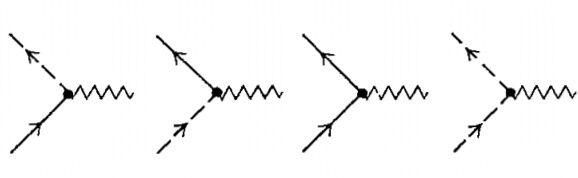
\includegraphics[width=10cm]{p2.jpg}
    \renewcommand{\figurename}{Fig.}
    \caption{Basic vertices for bosons}
    \label{img2}
\end{figure}

All diagrams of the first order term of the single particle Green's function 
$G'^{(1)}$ is shown in Fig.\ref{img3}, where only $\hat{W}_3$ and $\hat{W}_4$ 
contribute. Since $\hat{W}_1$, $\hat{W}_2$, $\hat{W}_5$, $\hat{W}_6$ don't conserve 
the number of particles and $\hat{W}_7$ will lead to diagrams involving holes.
\begin{figure}[H]
    \centering
    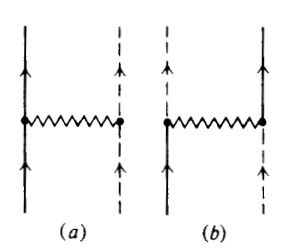
\includegraphics[width=6cm]{p3.jpg}
    \renewcommand{\figurename}{Fig.}
    \caption{All first-order contributions $G'^{(1)}$}
    \label{img3}
\end{figure}
\noindent The Feynman rules give (detailed calculation is at the end of this section.) 
\begin{equation}\label{Gp1}
    G^{\prime(1)}(q)=n_{0} \hbar^{-1} G^{0}(q)[W(0)+W(\mathbf{q})] G^{0}(q).
\end{equation}
\noindent The diagrams of second-order correction $G'^{(2)}$ are shown in 
Fig.\ref{img4}. The diagrams form $a$ to $e$ are of order $n_0^2$, while $f$ and 
$g$ are of order $n_0$.
\begin{figure}[H]
    \centering
    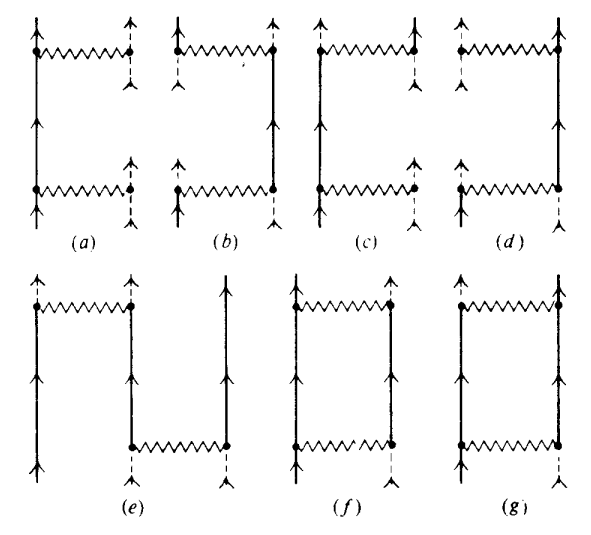
\includegraphics[width=11cm]{p4.png}
    \renewcommand{\figurename}{Fig.}
    \caption{All second-order contributions $G'^{(2)}$}
    \label{img4}
\end{figure}
\noindent\hrulefill

\noindent\hrulefill
\section{Dyson's Equations}
In Sec.3, we introduce the noncondensate single particle Green's function $G'$ 
and two anomalous Green's function $G'_{12}$ and $G'_{21}$. We represent them 
with thick arrows in Feynman diagrams (Fig.\ref{img5}). The direction of arrows 
indicates the direction of momentum flow in momentum space.
\begin{figure}[H]
    \centering
    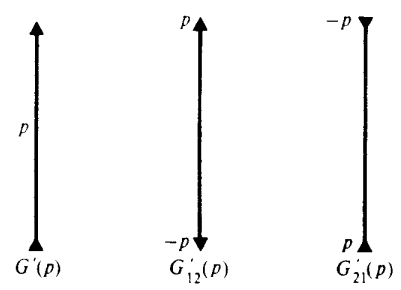
\includegraphics[width=6cm]{p5.png}
    \renewcommand{\figurename}{Fig.}
    \caption{noncondensate Green's functions for bosons}
    \label{img5}
\end{figure}
In addition, we define three kinds of irreducible self-energies $\Sigma^*_{11}(p)$, 
$\Sigma^*_{12}(p)$ and $\Sigma^*_{21}(p)$ (Fig.\ref{img6}), which are elements of 
matrix $\boldsymbol{\Sigma}^*(p)$
\begin{equation}
    \boldsymbol{\Sigma}^*(p)=\left(\begin{matrix}
        \Sigma^*_{11}(p) &\Sigma^*_{12}(p)\\
        \Sigma^*_{21}(p) &\Sigma^*_{11}(-p)
    \end{matrix}\right).
\end{equation}
The first one $\Sigma^*_{11}$ has one particle line entering and one leaving, while 
the others have two particle lines either coming out ($\Sigma^*_{12}$) or going in 
($\Sigma^*_{12}$).
\begin{figure}[H]
    \centering
    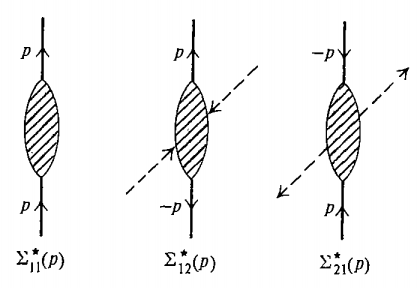
\includegraphics[width=8cm]{p6.png}
    \renewcommand{\figurename}{Fig.}
    \caption{Proper self energies for bosons}
    \label{img6}
\end{figure}
The Dyson equations for the system are shown in Fig.\ref{img7} and can be written 
in the momentum space:
\begin{subequations}
    \begin{align}
        &G'(p)=G^0(p)+G^0(p)\Sigma^*_{11}(p)G'(p)+G^0(p)\Sigma^*_{12}(p)G'_{21}(p)\label{Za}\\
        &G'_{12}(p)=G^0(p)\Sigma^*_{12}(p)G'(-p)+G^0(p)\Sigma^*_{11}(p)G'_{12}(p)\label{Zb}\\
        &G'_{21}(p)=G^0(-p)\Sigma^*_{21}(p)G'(p)+G^0(-p)\Sigma^*_{11}(-p)G'_{21}(p).\label{Zc}
    \end{align}
\end{subequations}
They can be written as a single matrix equation 
\begin{equation}\label{matrixGreen}
    \mathbf{G}'(p)=\mathbf{G}^0(p)+\mathbf{G}^0(p)\boldsymbol{\Sigma}^*(p)\mathbf{G}'(p)
\end{equation}
where 
\begin{equation}
    \mathbf{G}'(p)=\left(\begin{matrix}
        G'(p) &G'_{12}(p)\\
        G'_{21}(p) &G'(-p)
    \end{matrix}\right)\qquad
    \mathbf{G}^0(p)=\left(\begin{matrix}
        G^0(p) &0\\
        0 &G^0(-p)
    \end{matrix}\right)
\end{equation}
\begin{figure}[H]
    \centering
    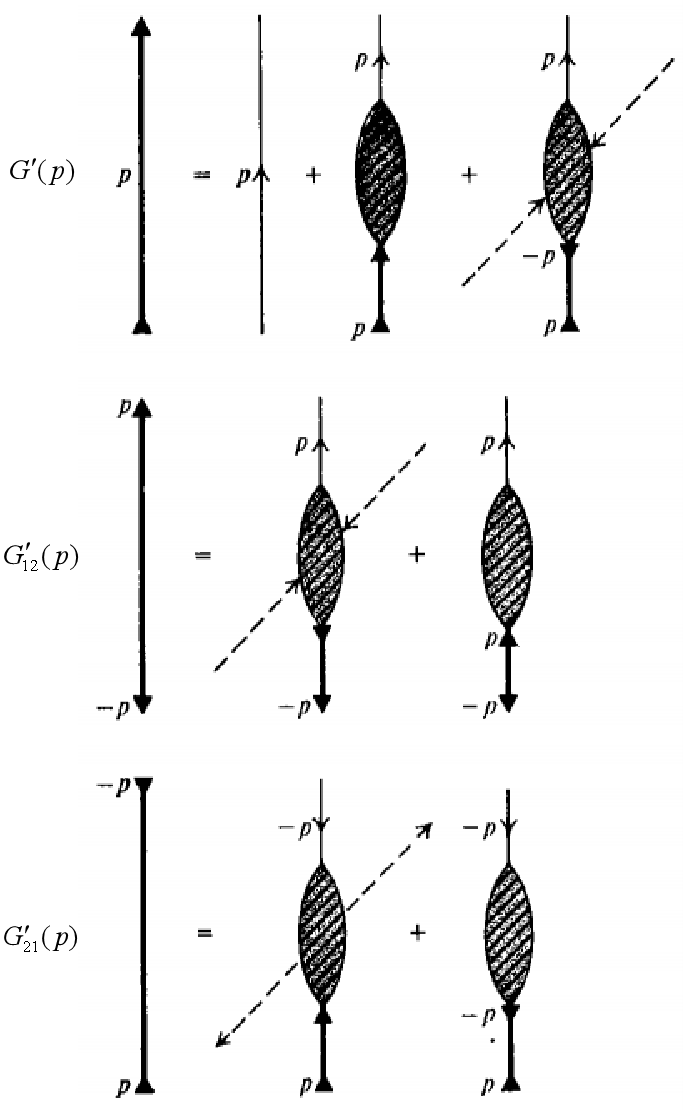
\includegraphics[width=8cm]{p7.png}
    \renewcommand{\figurename}{Fig.}
    \caption{Dyson's equations for bosons}
    \label{img7}
\end{figure}
The Eq.(\ref{matrixGreen}) can be rewritten as 
\begin{equation}
    \mathbf{G}'(p)=\big[\mathbf{G}^0(p)^{-1}-\boldsymbol{\Sigma}^*(p)\big]^{-1},
\end{equation}  
which yields 
\begin{equation}\label{eGp}
    \begin{split}
        &G'(p)=\frac{p_0+\omega_{\mathbf{p}}-\mu/\hbar+S(p)-A(p)}{D(p)}\\
        &G'_{12}(p)=-\frac{\Sigma^*_{12}(p)}{D(p)}\qquad
        G'_{21}(p)=-\frac{\Sigma^*_{21}(p)}{D(p)}
    \end{split}
\end{equation}
where
\begin{equation}
    D(p)=\left[p_{0}-A(p)\right]^{2}-\big[\omega_{\mathbf{p}}-\mu\hbar^{-1}+S(p)
    \big]^{2}+\Sigma_{12}^{\star}(p) \Sigma_{21}^{\star}(p)
\end{equation}
and 
\begin{equation}
    S(p)=\frac{1}{2}\left[\Sigma_{11}^*(p)+\Sigma_{11}^*(-p)\right]\quad 
    A(p)=\frac{1}{2}\left[\Sigma_{11}^*(p)-\Sigma_{11}^*(-p)\right].
\end{equation}
These equations are general, since all the Green's functions are expressed in terms 
of exact proper self-energies.
\section{Weakly Interaction Bose Gas}
We consider a weakly interaction Bose gas whose potential $W(\mathbf{r})$ has a 
well-defined Fourier transform $W(\mathbf{p})$. Since the interaction is weak, the 
self-energy only need to be evaluated to the lowest order. 
\begin{figure}[H]
    \centering
    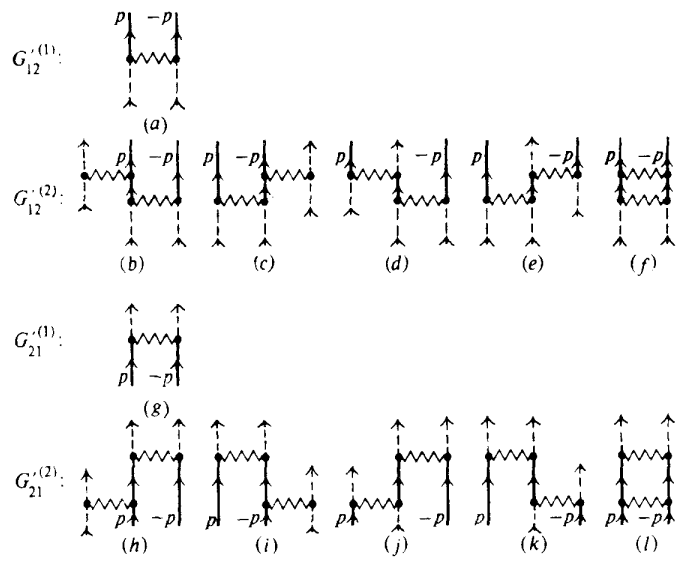
\includegraphics[width=13cm]{p8.png}
    \renewcommand{\figurename}{Fig.}
    \caption{All first and second contributions to $G'_{12}$ and $G'_{21}$.}
    \label{img8}
\end{figure}
\noindent According to Eq.(\ref{Gp1}), the lowest order of $\Sigma^{*(1)}_{11}$ is 
\begin{equation}
    \Sigma^{*(1)}_{11}(p)=n_0\hbar^{-1}[W(0)+W(\mathbf{p})]
\end{equation}
As is shown in Fig.\ref{img8}, the lowest orders of $G'_{12}$ and $G'_{21}$ are 
\begin{equation}
    \Sigma_{12}^*(p)=\Sigma_{21}^*(p)=n_{0}\hbar^{-1}W(\mathbf{p}).
\end{equation}
Note that $\Sigma_{12}^*(p)=\Sigma_{21}^*(-p)$, and both $\Sigma_{12}^*$ and 
$\Sigma_{21}^*$ are even functions of $p$. As the Eq.(\ref{equichemical}), the 
chemical potential is 
\begin{equation*}
    \mu=\bra*{O}\frac{\partial \hat{W}}{\partial N_0}\ket*{O}.
\end{equation*}
Expand it in seires in interaction representation:
\begin{equation}\label{mu1}
    \mu=\frac{\sum_{m=0}^{\infty}\left(\frac{-i}{\hbar}\right)^{m}\frac{1}{m!} 
    \int_{-\infty}^{\infty}dt_{1}\cdots\int_{-\infty}^{\infty}dt_{m}\bra*{0}T\big[
    \hat{K}_1(t_1)\cdots\hat{K}_1(t_m) \frac{\partial\hat{W}}{\partial N_0}\big]
    \ket*{0}}{\sum_{m=0}^{\infty}\left(\frac{-i}{\hbar}\right)^{m}\frac{1}{m!}
    \int_{-\infty}^{\infty}dt_{1}\cdots\int_{-\infty}^{\infty}dt_m\bra*{0}T\big[
    \hat{K}_{1}(t_1)\cdots\hat{K}_{1}(t_m)\big]\ket*{0}}
\end{equation}
As we know, the denominator will cancel the disconnected parts in the numerator, 
therefore Eq.(\ref{mu1}) can be rewritten 
\begin{equation}\label{mu1re}
    \mu=\sum_{m=0}^{\infty}\left(\frac{-i}{\hbar}\right)^{m} \frac{1}{m!}\int_
    {-\infty}^{\infty}dt_1\cdots \int_{-\infty}^{\infty}dt_m\bra*{0}T\Big[\hat{K}_1
    \left(t_{1}\right)\cdots\hat{K}_1(t_m) \frac{\partial\hat{W}}{\partial N_0}
    \Big] \ket*{0}_{\text{connected}}
\end{equation}
The lowest order is 
\begin{equation}
    \begin{split}
        \mu&=\bra*{0}\frac{\partial\hat{W}}{\partial N_0}\ket*{0}\\
        &=2 E_0N_0^{-1}+N_0^{-1}\bra*{0}\hat{W}_1+\hat{W}_2+\hat{W}_3+\hat{W}_4
        \ket*{0}+(2N_0)^{-1}\bra*{0}\hat{W}_5+\hat{W}_6\ket*{0}\\
        &=n_0W(0)
    \end{split}
\end{equation}
Therefore 
\begin{equation}\label{Hugenholtz}
    \mu=\hbar\Sigma^*_{11}(0)-\hbar\Sigma^*_{12}(0)
\end{equation}
In fact, this relation is satisfied for all orders and was derived by Hugenholtz 
and Pines.

Combinated with Eq.(\ref{eGp}), The noncondensate Green's function can be written 
as 
\begin{equation}\label{weakGp1}
    \begin{aligned}
        &G'(p)=\frac{p_{0}+\hbar^{-1}\left[\epsilon_{\mathbf{p}}^{0}+n_0
        W(\mathbf{p})\right]}{p_{0}^{2}-\left(E_{\mathbf{p}}/\hbar\right)^{2}}\\
        &G_{12}^{\prime}(p)=G_{21}^{\prime}(p)=\frac{-\hbar^{-1}n_0W(\mathbf{p})}
        {p_{0}^{2}-\left(E_{\mathbf{p}} / \hbar\right)^2}
    \end{aligned}
\end{equation} 
where
\begin{equation}
    \begin{aligned}
        E_{p} &=\big\{\big[\epsilon_{\mathbf{p}}^{0}+n_{0} W(\mathbf{p})\big]^{2}
        -\big[n_{0} W(\mathbf{p})\big]^{2}\big\}^{\frac{1}{2}} \\
        &=\big\{{\epsilon_{\mathbf{p}}^0}^2+2\epsilon_{\mathbf{p}}^0n_0
        W(\mathbf{p})\big\}^{\frac{1}{2}}
        \end{aligned}
\end{equation} 
It is convenient to seperate the two poles in Eq.(\ref{weakGp1})
\begin{subequations}
    \begin{align}
        &G'(p)=\frac{u_{\mathbf{p}}^2}{p_0-E_{\mathbf{p}}/\hbar+i\eta}-
        \frac{v_{\mathbf{p}}^{2}}{p_{0}+E_{\mathbf{p}} /\hbar-i\eta}\label{Za}\\
        &G_{12}'(p)=G_{21}'(p)=\frac{-u_{\mathbf{p}}v_{\mathbf{p}}}{p_{0}-
        E_{\mathbf{p}}/\hbar+i \eta}+\frac{u_{\mathbf{p}}v_{\mathbf{p}}}{p_0+
        E_{\mathbf{p}}/\hbar-i\eta}\label{Zb}
        \end{align}
\end{subequations}
Where
\begin{equation}
    \begin{aligned}
        u_{\mathbf{p}}=\Big\{\frac{1}{2} E_{\mathbf{p}}^{-1}\big[\epsilon_{\mathbf{p}}^{0}
        +n_0W(\mathbf{p})\big]+\frac{1}{2}\Big\}^{\frac{1}{2}}\\
        v_{\mathbf{p}}=\Big\{\frac{1}{2}E_{\mathbf{p}}^{-1}\big[\epsilon_{\mathbf{p}}
        ^{0}+n_{0}W(\mathbf{p})\big]-\frac{1}{2}\Big\}^{\frac{1}{2}}.
    \end{aligned}  
\end{equation}
In long-wavelength limit, the excitation spectrum $E_\mathbf{p}$ display a linear 
dispersion like phonons
\begin{equation}
    E_{\mathbf{p}}\approx \hbar|\mathbf{p}|\Big(\frac{n_0W(0)}{m}\Big)^{\frac{1}{2}}
    \qquad |\mathbf{p}|\rightarrow 0.
\end{equation}
According to Eq.(\ref{N}), since only the pole at $p_0=-E_\mathbf{p}/\hbar+i\eta$ contributes, 
the number of particles is 
\begin{equation}\label{N1}
    n=n_{0}+(2 \pi)^{-3} \int d^{3} p\ v_{\mathbf{p}}^{2}
\end{equation}
\section{Dilute Bose Gas With Repulsive Cores}
We consider a dilute Bose gas, in which $na^3\ll 1$. $a$ is the scattering length.
The potential $W(\mathbf{r})$ no longer has a well-defined Fourier transform. 
We need to calculate the sum of a selected class of diagrams to obtain the 
self-energy(Fig.\ref{img9}).
\begin{figure}[H]
    \centering
    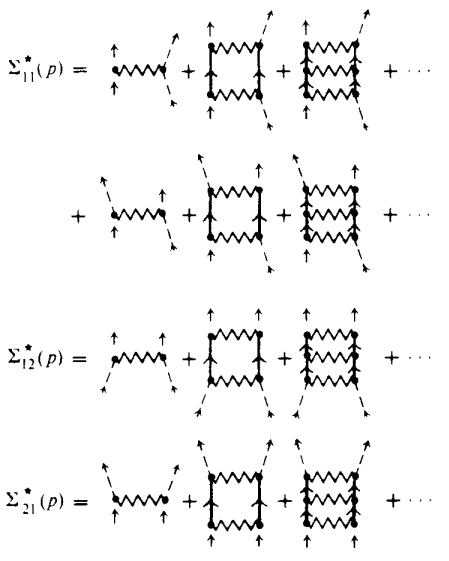
\includegraphics[width=9cm]{p9.png}
    \renewcommand{\figurename}{Fig.}
    \caption{Ladder summation for proper self-energy}
    \label{img9}
\end{figure}
\noindent Bethe-Salpeter equation:
\begin{equation}
    \begin{aligned}
        \chi\left(\mathbf{p}, \mathbf{p}',P\right)=(2\pi)^{3}\delta(\mathbf{p}-
        \mathbf{p}')+\big(\epsilon+&2m\mu \hbar^{-2}-p^{2}+i\eta\big)^{-1}(2\pi)^{-3}\\
        &\times\int d^3q\ v(\mathbf{q})\chi\left(\mathbf{p}-\mathbf{q},\mathbf{p}',P\right)
        \end{aligned}
\end{equation}
\begin{equation}
    m\hbar^{-2}\Gamma\left(\mathbf{p}, \mathbf{p}',P\right)=(2\pi)^{-3}\int d^3q\ v
    (\mathbf{q})\chi\left(\mathbf{p}-\mathbf{q}, \mathbf{p}', P\right).
\end{equation}
$\Gamma(p_1p_2;p_3p_4)$ is the effective two-particle interaction.
\begin{figure}[H]
    \centering
    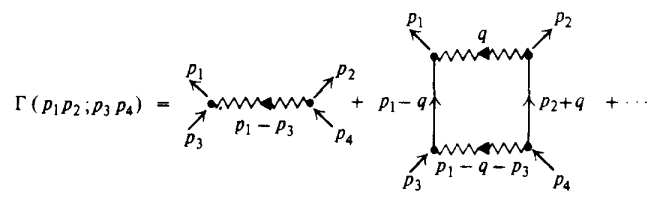
\includegraphics[width=12cm]{p10.png}
    \renewcommand{\figurename}{Fig.}
    \caption{Ladder summation for effective interaction}
    \label{img10}
\end{figure}
\noindent We set $P=p_1+p_2=p_3+p_4$ as the center of mass momentum, and 
\begin{equation*}
    p=\frac{1}{2}(p_1-p_2)\qquad p'=\frac{1}{2}(p_3-p_4)
\end{equation*}
as the relative momenta, then 
\begin{equation*}
    \Gamma(p_1p_2;p_3p_4)\rightarrow\Gamma(\mathbf{p}, \mathbf{p}',P).
\end{equation*}
In dilute Bose systems, the solution is 
\begin{equation}
    \begin{aligned}
        m\hbar^{-2} \Gamma(\mathbf{p},\mathbf{p}',P)=&\tilde{f}(\mathbf{p},
        \mathbf{p}')+\int\frac{d^3 k}{(2\pi)^3}\tilde{f}(\mathbf{p},\mathbf{k})\\
        &\times\bigg(\frac{1}{\epsilon+2m\mu/\hbar^2-k^2+i\eta}+\frac{1}{k^2-p'^2-i\eta}
        \bigg)\tilde{f}(\mathbf{p}',\mathbf{k})^*
        \end{aligned}
\end{equation}
where $\tilde{f}(\mathbf{p},\mathbf{k})$ is the scattering amplitude for a transform from an 
incident momentum $k$ to a final momentum $p$.

In the long-wavelength limit ($|\mathbf{p}|\rightarrow0$), the leading term reduces to 
\begin{equation}
    \Gamma(\mathbf{p},\mathbf{p}',P)\rightarrow 4\pi a\hbar^2m^{-1} \qquad
    |\mathbf{p}|a\ll 1,\ |\mathbf{p}'|a\ll 1
\end{equation}
where $a$ is the s-wave scattering length. Thus we have 
\begin{equation}
    \begin{split}
        &\hbar \Sigma_{11}^*(p)=n_{0} \Gamma\big({\textstyle\frac{1}{2}}\mathbf{p},
        {\textstyle\frac{1}{2}}\mathbf{p}, P\big)+n_0\Gamma\big({-\textstyle\frac{1}{2}}
        \mathbf{p},{\textstyle\frac{1}{2}}\mathbf{p},P\big)\approx8\pi n_0a\hbar^2m^{-1}\\
        &\hbar \Sigma_{12}^*(p)=n_0\Gamma(\mathbf{p},0,0)\approx 4\pi n_0a \hbar^2m^{-1}\\
        &\hbar \Sigma_{21}^*(p)=n_0\Gamma(0,\mathbf{p},0) \approx 4\pi n_0a\hbar^2m^{-1}.
    \end{split}     
\end{equation}
We again have $\Sigma^*_{12}(p)=\Sigma^*_{21}(p)$.

As Eq.(\ref{mu1re})
\begin{equation*}
    \mu=\sum_{m=0}^{\infty}\left(\frac{-i}{\hbar}\right)^{m} \frac{1}{m!}\int_
    {-\infty}^{\infty}dt_1\cdots \int_{-\infty}^{\infty}dt_m\bra*{0}T\Big[\hat{K}_1
    \left(t_{1}\right)\cdots\hat{K}_1(t_m) \frac{\partial\hat{V}}{\partial N_0}
    \Big] \ket*{0}_{\text{connected}},
\end{equation*}
we can also represent $\mu$ as summation of ladder diagrams (Fig.\ref{img11}).
\begin{figure}[H]
    \centering
    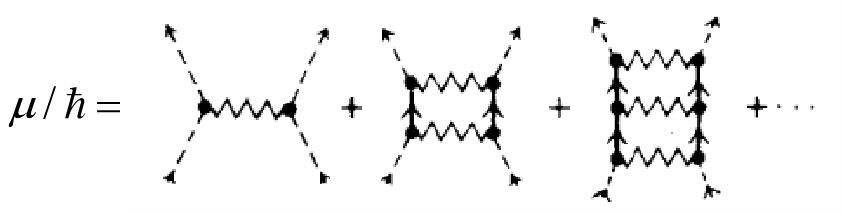
\includegraphics[width=9cm]{p11.png}
    \renewcommand{\figurename}{Fig.}
    \caption{Ladder summation for chemical potential}
    \label{img11}
\end{figure}
\noindent Therefore the approximate chemical potential is 
\begin{equation}
    \mu=n_0\Gamma(0,0,0)\approx 4\pi n_0a\hbar^2m^{-1}
\end{equation}
which also satisfies the Hugenholtz-Pines relation (Eq.(\ref{Hugenholtz})). Then the 
single particle Green's function when $|\mathbf{p}|a\ll 1$ is 
\begin{equation}
    G^{\prime}(p)=\frac{u_{\mathbf{p}}^{2}}{p_0-E_{\mathbf{p}}/\hbar+i\eta}-\frac
    {v_{\mathbf{p}}^{2}}{p_{0}+E_{\mathbf{p}} / \hbar-i \eta}
\end{equation}
where 
\begin{equation}
    \begin{split}
        &u_{\mathbf{p}}^{2}=\frac{1}{2}\big[E_{\mathbf{p}}^{-1}\big(\epsilon_{\mathbf{p}}^{0}+4\pi
        n_0a\hbar^{2} m^{-1}\big)+1\big]\\
        &v_{\mathbf{p}}^{2}=\frac{1}{2}\big[E_{\mathbf{p}}^{-1}\big(\epsilon_{\mathbf{p}}^0+4\pi
        n_{0} a \hbar^{2} m^{-1}\big)-1\big]
    \end{split}
\end{equation}
and 
\begin{equation}
    E_{\mathbf{p}}=\big({\epsilon_\mathbf{p}^0}^2+8\pi n_0a\hbar^{2}\epsilon_{
    \mathbf{p}}^0m^{-1}\big)^{\frac{1}{2}}
\end{equation}
According to Eq.(\ref{N1}), the total density is 
\begin{equation}
    \begin{aligned}
        n&=n_0+\frac{1}{2}(2 \pi)^{-3}\int d^3 p\big[E_{\mathbf{p}}^{-1}
        \big(\epsilon_{\mathbf{p}}^0+4\pi n_0a\hbar^2m^{-1}\big)-1\big] \\
        &=n_0+\frac{8}{3}\pi^{-\frac{1}{2}}(n_0a)^{\frac{1}{2}}\approx n_0+
        \frac{8}{3}\pi^{-\frac{1}{2}}(na)^{\frac{3}{2}}
        \end{aligned}
\end{equation}
\begin{equation}
    \frac{n-n_0}{n}=\frac{8}{3}\left(\frac{na^3}{\pi}\right)^{\frac{1}{2}}\ll 1
\end{equation}
According to Eq.(\ref{E}), the energy is 
\begin{equation}
    \begin{aligned}
        E V^{-1}=&\frac{1}{2}\mu n+\left(32\pi^{3}\right)^{-1}\int d^3 p
        \left(\epsilon_{\mathbf{p}}^{0}-E_{\mathbf{p}}\right)\left[E_{\mathbf{p}}
        ^{-1}\left(\epsilon_{\mathbf{p}}^0+4\pi n_0a\hbar^2m^{-1}\right)-1\right]\\
        =&\frac{1}{2}\mu n+\hbar^{2}\left(8\pi n_0a\right)^{\frac{5}{2}}\left(16
        \pi^{2} m\right)^{-1}\int_0^{\infty}y^{2}dy\big[\left(2 y^{3}+3 y\right)
        \left(y^{2}+2\right)^{-\frac{1}{2}}-2 y^{2}-1\big] \\
        =& \frac{1}{2} \mu n-\frac{64 \pi^{\frac{1}{2}}\left(n_{0} a\right)^{\frac
        {1}{2}} \hbar^{2}}{15 m}\approx\frac{1}{2}\mu n-\frac{64\pi^{\frac{1}{2}}
        (n a)^{\frac{5}{2}} \hbar^{2}}{15 m}
        \end{aligned}
\end{equation}
We assume that 
\begin{equation}
    \mu=4 \pi n a \hbar^{2} m^{-1}\big[1+\alpha(n a^{3})^{\frac{1}{2}}\big]
\end{equation}
\begin{equation}
    \Rightarrow\frac{E}{V}=\frac{2\pi n^2a\hbar^{2}}{m}\bigg[1+\alpha(n a^3)^{
    \frac{1}{2}}-\frac{32}{15}\left(\frac{na^3}{\pi}\right)^{\frac{1}{2}}\bigg].
\end{equation} 
With the thermodynamic relation
\begin{equation}
    \mu=\left(\frac{\partial E}{\partial N}\right)_{V}=\frac{1}{V}
    \frac{\partial E}{\partial n}=\frac{4\pi na\hbar^{2}}{m}\bigg[1+\frac{5}{4}
    \alpha(na^3)^{\frac{1}{2}}-\frac{8}{3}\left(\frac{na^3}{\pi}\right)^{\frac{1}
    {2}}\bigg]
\end{equation}
we can determine that $\alpha=32/3\pi^{\frac{1}{2}}$ and 
\begin{align}
    \frac{E}{V}=\frac{2\pi n^2a\hbar^{2}}{m}\bigg[1+\frac{128}{15}\left(\frac{na^3}
    {\pi}\right)^{\frac{1}{2}}\bigg]\label{Lee}\\
    \mu=\frac{4\pi na\hbar^2}{m}\bigg[1+\frac{32}{3}\left(\frac{na^3}{\pi}\right)
    ^{\frac{1}{2}}\bigg]
\end{align}
Eq.(\ref{Lee}) determines the leading correction to the ground state energy, and 
was first obtained by Lee and Yang. 

\end{document}